\paragraph{Sơ đồ tuần tự luồng đăng nhập bằng email \& password}

Luồng nghiệp vụ này mô tả
quá trình người dùng
sử dụng tài khoản đã được kích hoạt trước
đó để đăng nhập bằng phương thức POST trả về dữ liệu định dạng JSON,
sau đó chuyển sang bước xác thực MFA để nâng cấp phiên làm việc trước khi truy cập hệ thống.

\begin{figure}[H]
\centering
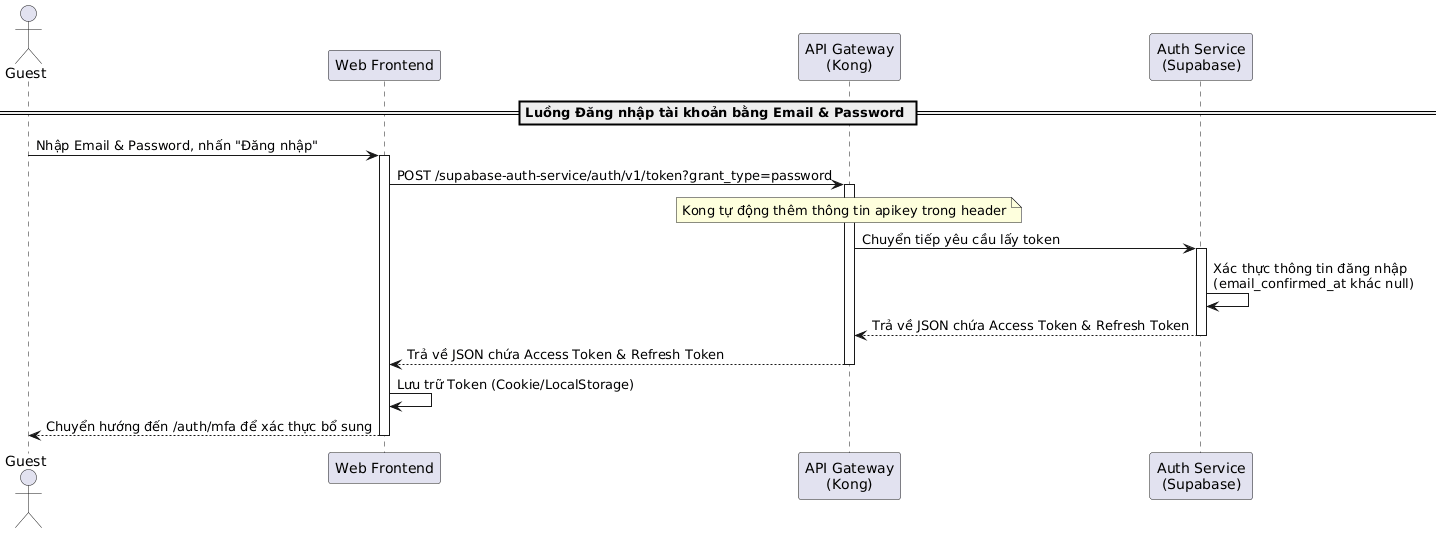
\includegraphics[width=0.95\textwidth]{contents/Sequence/UML-Sequence-UserEmailPasswordLogin.png}
\caption{Sơ đồ tuần tự luồng đăng nhập bằng email \& password}
\end{figure}

\begin{table}[H]
\centering
\renewcommand{\arraystretch}{1.3}

\begin{tabular}{|l|l|p{5cm}|}
\hline
\textbf{Thành phần} & \textbf{Phân loại} & \textbf{Vai trò trong hệ thống} \\ \hline
Guest & Actor & Khách vãng lai đăng nhập bằng tài khoản sẵn có. \\ \hline
Web Frontend & Component & Giao diện web Next.js. \\ \hline
API Gateway (Kong) & Component & Cổng API chuyển tiếp các yêu cầu API. \\ \hline
Auth Service (Supabase) & Microservice & Xác thực thông tin tài khoản và trả trực tiếp dữ liệu token dạng JSON. \\ \hline
\end{tabular}
\caption{Các thành phần tham gia luồng đăng nhập bằng email \& password}
\end{table}

\subparagraph{Mô tả tổng quan}

\begin{itemize}

\item \textbf{Nhập thông tin đăng nhập:}
Người dùng điền
địa chỉ thư điện tử và mật khẩu,
sau đó chọn đăng nhập trên giao diện.

\item \textbf{Yêu cầu đăng nhập:}
Giao diện gửi yêu cầu đăng nhập
trực tiếp qua cổng API đến Auth Service.

\item \textbf{Kiểm tra tài khoản:}
Auth Service kiểm tra thông tin đăng nhập
và đảm bảo tài khoản
đã hoàn tất xác thực thư điện tử trước đó.

\item \textbf{Cấp mã phiên:}
Nếu thông tin chính xác,
Auth Service tạo cặp mã đăng nhập
và mã làm mới phiên đăng nhập gửi về qua cổng API.

\item \textbf{Xác thực bổ sung:}
Cổng API chuyển tiếp thông tin đăng nhập về giao diện.
Giao diện thực hiện lưu trữ
các mã đăng nhập cục bộ
và chuyển hướng người dùng sang trang xác thực hai lớp.
Sau khi hoàn thành xác thực hai lớp đạt mức bảo mật yêu cầu,
người dùng được chuyển hướng vào màn hình trò chuyện chính.
\end{itemize}
